
\documentclass{beamer}
\usepackage{setspace}
\usepackage{gensymb}
\usepackage{caption}
%\usepackage{multirow}
%\usepackage{multicolumn}
%\usepackage{subcaption}
%\doublespacing
\singlespacing
\usepackage{csvsimple}
\usepackage{amsmath}
\usepackage{multicol}
%\usepackage{enumerate}
\usepackage{amssymb}
%\usepackage{graphicx}
\usepackage{newfloat}
%\usepackage{syntax}
\usepackage{listings}
%\usepackage{iithtlc}
\usepackage{color}
\usepackage{tikz}
\usetikzlibrary{shapes,arrows}



%\usepackage{graphicx}
%\usepackage{amssymb}
%\usepackage{relsize}
%\usepackage[cmex10]{amsmath}
%\usepackage{mathtools}
%\usepackage{amsthm}
%\interdisplaylinepenalty=2500
%\savesymbol{iint}
%\usepackage{txfonts}
%\restoresymbol{TXF}{iint}
%\usepackage{wasysym}
\usepackage{amsthm}
\usepackage{mathrsfs}
\usepackage{txfonts}
\usepackage{stfloats}
\usepackage{cite}
\usepackage{cases}
\usepackage{mathtools}
\usepackage{caption}
\usepackage{enumerate}	
\usepackage{enumitem}
\usepackage{amsmath}
%\usepackage{xtab}
\usepackage{longtable}
\usepackage{multirow}
%\usepackage{algorithm}
%\usepackage{algpseudocode}
\usepackage{enumitem}
\usepackage{mathtools}
\usepackage{hyperref}
%\usepackage[framemethod=tikz]{mdframed}
\usepackage{listings}
    %\usepackage[latin1]{inputenc}                                 %%
    \usepackage{color}                                            %%
    \usepackage{array}                                            %%
    \usepackage{longtable}                                        %%
    \usepackage{calc}                                             %%
    \usepackage{multirow}                                         %%
    \usepackage{hhline}                                           %%
    \usepackage{ifthen}                                           %%
  %optionally (for landscape tables embedded in another document): %%
    \usepackage{lscape}     


\usepackage{url}
\def\UrlBreaks{\do\/\do-}


%\usepackage{stmaryrd}


%\usepackage{wasysym}
%\newcounter{MYtempeqncnt}
\DeclareMathOperator*{\Res}{Res}
%\renewcommand{\baselinestretch}{2}
\renewcommand\thesection{\arabic{section}}
\renewcommand\thesubsection{\thesection.\arabic{subsection}}
\renewcommand\thesubsubsection{\thesubsection.\arabic{subsubsection}}

%\renewcommand\thesectiondis{\arabic{section}}
%\renewcommand\thesubsectiondis{\thesectiondis.\arabic{subsection}}
%\renewcommand\thesubsubsectiondis{\thesubsectiondis.\arabic{subsubsection}}

% correct bad hyphenation here
\hyphenation{op-tical net-works semi-conduc-tor}

%\lstset{
%language=C,
%frame=single, 
%breaklines=true
%}

%\lstset{
	%%basicstyle=\small\ttfamily\bfseries,
	%%numberstyle=\small\ttfamily,
	%language=Octave,
	%backgroundcolor=\color{white},
	%%frame=single,
	%%keywordstyle=\bfseries,
	%%breaklines=true,
	%%showstringspaces=false,
	%%xleftmargin=-10mm,
	%%aboveskip=-1mm,
	%%belowskip=0mm
%}

%\surroundwithmdframed[width=\columnwidth]{lstlisting}
\def\inputGnumericTable{}                                 %%
\lstset{
%language=C,
frame=single, 
breaklines=true,
columns=fullflexible
}


\begin{document}
\title{\textbf{Splines}}   
\author{\textit{Raktim Gautam Goswami (EE17BTECH11051) \newline Abhishek Bairagi (EE17BTECH11004)}} 
\date{\today} 

\frame{\titlepage} 

\frame{\frametitle{Table of contents}\tableofcontents} 


\section{Finding best fit for a data } 
\frame{\frametitle{Problem Statement} 
Finding best fit for a data

}

\section{Figure 1}
\frame{\frametitle{Figure 1}
Suppose we are given few points
\begin{figure}
  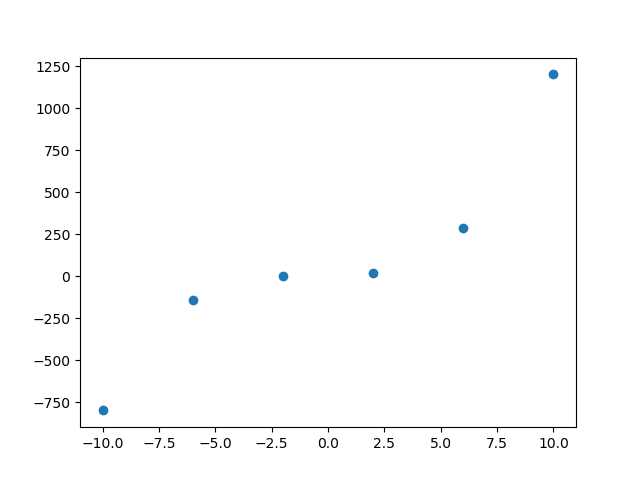
\includegraphics[width=200pt]{./Figs/Figure_1.png}
  
  \label{figure}
\end{figure}
}
\section{Figure 2}
\frame{\frametitle{Figure 2}
They can be joined linearly 
\begin{figure}
  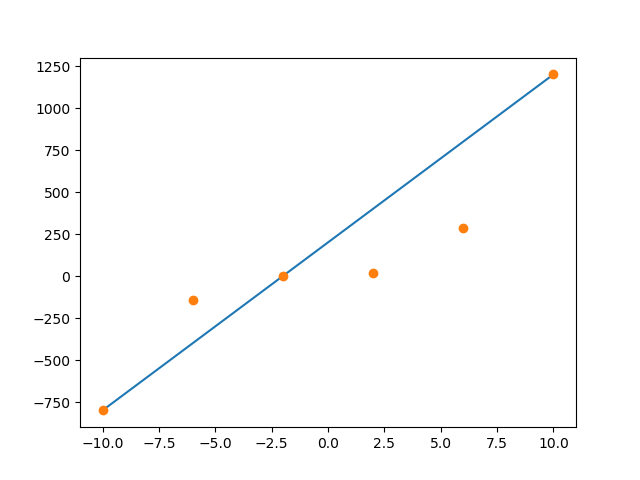
\includegraphics[width=200pt]{./Figs/Figure_2.png}
 
  \label{figure}
\end{figure}
}
\section{Figure 3}
\frame{\frametitle{Figure 3}

\begin{figure}
  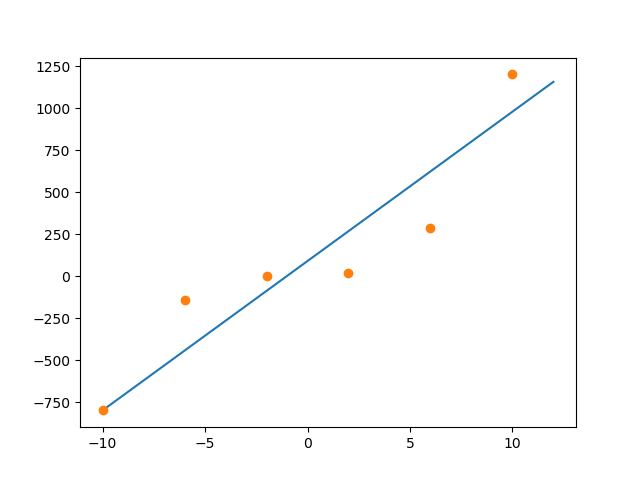
\includegraphics[width=200pt]{./Figs/Figure_3.png}
  
  \label{figure}
\end{figure}
}
\section{Figure 4}
\frame{\frametitle{Figure 4}
In a better way
\begin{figure}
  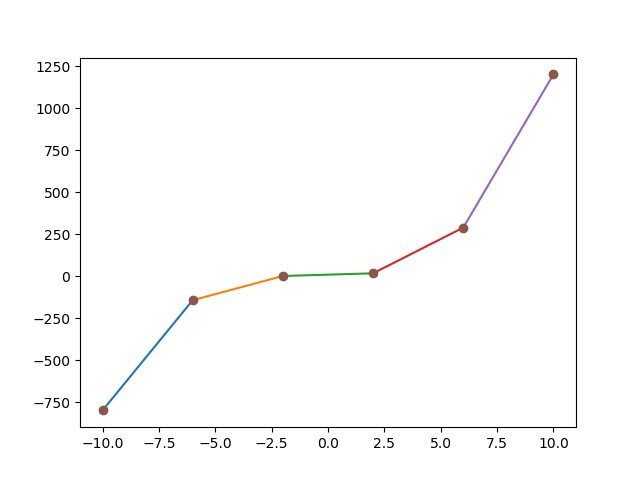
\includegraphics[width=200pt]{./Figs/Figure_4.png}
 
  \label{figure}
\end{figure}
}
\section{Figure 5}
\frame{\frametitle{Figure 5}

\begin{figure}
  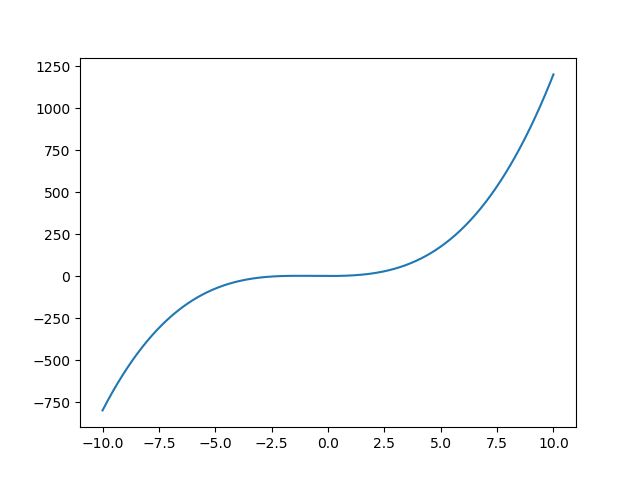
\includegraphics[width=200pt]{./Figs/Figure_5.png}
  
  \label{figure}
\end{figure}
}


\section{Options that we have} 
\frame{\frametitle{Options that we have}
\begin{itemize}
\item \textbf{1. nth order polynomial}\newline\newline
\item \textbf{2. Lagrange's coefficient polynomial}\newline\newline
\begin{equation}
\sum_{k=0}^{N} [Y_{k}L_{n,k}(x)]
\end{equation}
\begin{equation}
L_{n,k}(x) = \frac{(x-x_{0})(x-x_{1})...(x-x_{k-1})(x-x_{k})...(x-x_{n})}{(x_{k}-x_{0})(x_{k}-x_{1})....(x_{k}-x_{k-1})(x_{k}-x_{k+1})....(x_{k}-x_{n})}
\end{equation}
\item \textbf{3. Splines}\newline\newline
\end{itemize} 
}

\section{Splines}
\frame{\frametitle{Types of splines}
\begin{itemize}
\item \textbf{Piecewise cubic spines}\newline\newline\newline\newline
\item \textbf{Smoothing splines}



\end{itemize} 
}
\section{Cubic splines}
\frame{\frametitle{Cubic splines}
\begin{itemize}
\item Each pair of adjacent known points are assumed to be lying on a cubic curve.
\item At each known point, the two cubic parts from both sides are chosen such that the overall function is twice differentiabe at that point.
\item At the first and last given point, it is assumed that the doube derivative is zero.
\item Between any two given points, the cubic function is expressed as\newline
$S_{k}(x) = S_{k,0} + S_{k,1}(x-x_{k}) + S_{k,2}(x-x_{k})^{2} + S_{k,3}(x-x_{k})^{3}$
\end{itemize}
}




\section{How to find the coefficients} 
\frame{\frametitle{How to find the coefficients}
\begin{itemize}
\item \text{On comparing we get}\newline\newline
\begin{equation}
s_{k}(x_{k}) = y_{k}
\end{equation}
\begin{equation}
s_{k}(x_{k+1}) = s_{k+1}(x_{k+1})
\end{equation}
\begin{equation}
s^{'}_{k}(x_{k+1}) = s^{'}_{k+1}(x_{k+1})
\end{equation}
\begin{equation}
s^{''}_{k}(x_{k+1}) = s^{''}_{k+1}(x_{k+1})
\end{equation}
\begin{equation}
s^{''}_{k}(x_{0}) = 0
\end{equation}
\begin{equation}
s^{''}_{n}(x_{n}) = 0
\end{equation}
\end{itemize} 
}



\end{document}
